%%%%%%%%%%%%%%%%%%%%%%%%%%%%%%%%%%%%%%%%%%%%%%%%%%%%%%%%%%%%%%%%%%%%%%%%%%%%%%%%
%2345678901234567890123456789012345678901234567890123456789012345678901234567890
%        1         2         3         4         5         6         7         8

\documentclass[letterpaper, 10 pt, conference]{ieeeconf}  % Comment this line out if you need a4paper

%\documentclass[a4paper, 10pt, conference]{ieeeconf}      % Use this line for a4 paper

\IEEEoverridecommandlockouts                              % This command is only needed if
                                                          % you want to use the \thanks command

\overrideIEEEmargins                                      % Needed to meet printer requirements.

% See the \addtolength command later in the file to balance the column lengths
% on the last page of the document

% The following packages can be found on http:\\www.ctan.org
%\usepackage{graphics} % for pdf, bitmapped graphics files
%\usepackage{epsfig} % for postscript graphics files
%\usepackage{mathptmx} % assumes new font selection scheme installed
%\usepackage{times} % assumes new font selection scheme installed
%\usepackage{amsmath} % assumes amsmath package installed
\usepackage{graphicx}

%\usepackage{amssymb}  % assumes amsmath package installed

\title{\LARGE \bf Interprocess Communication for Robotics Applications
}

\author{Edward M. Roderick$^{*}$
\thanks{$^{*}$Author is affilited with George Mason University, Fairfax VA, 22030, USA. {\tt\small eroderi2@gmu.edu.}}%
}
\begin{document}



\maketitle
\thispagestyle{empty}
\pagestyle{empty}


\begin{abstract}

Modern robotic systems are developed as a collection of independent processes. For these processes to function together, an interprocess communication system (IPC) must be implemented. Many prebuilt systems are available and this paper presents four popular options (Sockets, ZeroMQ, ACH, and ROS) as candiates for robotics. An analysis is presented for each based on communication latency and design metrics as applied to robotics. An example design is presented with analysis of the IPC selection process.

\end{abstract}





\section{INTRODUCTION}

As modern robotic systems grow in complexity, it becomes increasingly beneficial to implement a multi-process control system. This provides a modular system architecture. A modular architecture protects the overall system from individual components failing\cite{ACHLIBRARY}. Critical system processes can be allocated additional resources to ensure continued operation during a partial system failure. By predefining the inputs and outputs for each subsystem, multiple teams of designers can use differing languages, allowing for optimization of each task. Additionally, the overall system can be distributed across a variety of hardware (full computers, single board computers, micro-controllers)\cite{REALTIMEACH, EMBEDDEDROS, ACHHUBO}. 

Many IPC options are available to designers and each must be evaluated on a per system basis to determine the best candidate. This paper will focus on evaluating several mainstream options and how they apply to design metrics of robotic systems. As robots operate in real time, the latency and data integrity of each communication step is of critical importance\cite{IPCS}. For complex systems (humanoids, robots operating in proximity with humans, etc) with multiple processes running concurrently, communication delay can results in actuators responding to obsolete data\cite{ACHHUBO}. This paper serves to provide a guide to evaluating the capabilities of Sockets, Shared Memory, and ROS. 

\section{BACKGROUND}

\subsection{ACH (Shared Memory)}

POSIX IPC offers three types of messages: streams, datagrams and shared memory. For the real time robotics application, it is important to ensure that the IPC system is non head of line blocking as the most recent sensor data will take priority over previously acquired data. Streams suffers from head of line blocking and is thus not a desirable method for robotics. Datagrams utilize a data buffer that when full, loses any new data. This is particularly problematic as the robot would routinely lose important data. Shared memory is the fastest method of the POSIX suite and will provide the most current data by overwriting any old information stored. Unfortunately this method is susceptible to synchronization issues and further considerations must be taken in code which would reduce its reusability and complexity. Furthermore, for a realtime system, none of the POSIX IPC methods allow any methods of priority inheritance which is critical to allow high priority systems to access data first.

The ACH system allows the system to create multiple data channels to send data between processes. Each channel consists of two circular buffers: a data buffer and an index buffer. The two buffers are written in a channel specific POSIX shared memory file. By storing the data buffers in shared memory, the synchronization issue can be solved once for the entire channel via a mutex, allowing each reader process to poll the channel or wait for new data to be posted. This also prevents starvation and allows for priority inheritance between the real time processes.

A case study is presented \cite{REALTIMEACH} in which a balancing bipedal robot was developed with many different processes and ACH channels. The study details how the multiprocess approach allows for high priority processes (like balancing in this case) to stay alive in the event that other processes fail (ie computer vision). This approach also allowed processes to be distributed between smaller microcontrollers to drive servomotors to higher powered computers to process computer vision. SPIN simulations were run to benchmark the ACH system and it was shown that performance is identical to POSIX for single readers and receivers and the majority of the latency is a product of context switches. 



\subsection{Sockets: TCP and UDP}

placeholder for tcp and udp backgrounds

\subsection{ZeroMQ}

ZeroMQ (ZMQ) is a messaging system that extends on the foundations of sockets. It provides an additional abstraction layer over TCP by sending messages to a system topology instead of specific IP addresses. ØMQ prevents sending to specific IP addresses by design. The available messaging patterns is open ended, popular systems include publish/subscribe and request/reply. Only one messaging pattern is allowed for a topology and they cannot be interconnected. 

\begin{figure}[p]
    \centering
    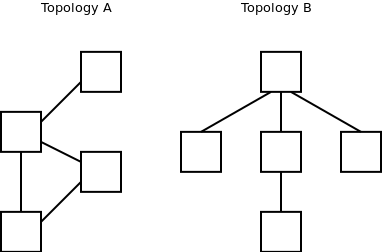
\includegraphics{zmqtopology}
    \caption{test}
    \label{test}
\end{figure}

This is essential to providing guarantees that data will arrive at its intended location. ØMQ separates its stack into end to end and hop by hop layers. Unlike TCP/IP, each ØMQ end to end protocol has its own hop by hop protocol\cite{ZMQTHEORY}. This allows each specific messaging pattern to have their own routing functionality. This allows bidirectional messages to be sent to specific nodes in the topology. Each intermediary node can determine if downstream sections of the network are unreachable and can signal the original client to resend now or wait until connectivity has been reestablished. 

With multicore processors being commonplace in today’s market and the growing availability of multicore processors in commercially available embedded systems there is a need for efficiently written multithreaded code. Current methods of dealing with the issues that arise from multithreading (synchronization, starvation, priority inversion) are difficult to learn and do not scale well as the number of available cores increases. By creating code with too many locks, threads can block one another and the system can perform inconsistently depending on what system the program is running on. Writing lock free code can become susceptible to processors reordering instructions and the code again performing inconsistently. These multithreading approaches are API based and incorrect usage can often result in multiple threads blocking each other and the program essentially running as a single threaded process. 
ZeroMQ provides a solution to these issues by abstracting the more difficult lock free multithreading code behind its native message passing techniques and achieves simple multithreading by sending messages between threads. Being based on BSD Sockets, the code implementation is simple and intuitive for existing programmers, as well as being available for a multitude of programming languages. ZeroMQ is infinitely scalable as the number of available cores increases without any rewriting of existing code.

\subsection{ROS}

With the growing availability of cheap ARM processor systems, versions of ROS are being developed to provide a lower cost design than the traditional full-fledged Linux pc. ROS subsystems can be distributed over multiple ARM systems, allowing for more design flexibility, lower power consumption, and improved scalability. ROS allows for higher level systems to be separated from real time subsystems and other system critical functions. This allows for high priority systems to be simplified to reduce risk of failure. ROS was designed to support higher level robot functions instead of the control of individual motors/sensors/etc. Much of the integration of subsystems is left to the design as ROS does not support fieldbuses. 

Three architecture styles exist for the designing to embed the ROS system: Embedded PC, Proprietary system with interface, or use of ROS messaging and APIs. The embedded PC would require all control hardware of subsystems to be fitted to the PC itself. This provides smooth integration with ROS, but fails to offer real hard time support. Entire existing robots can be managed from ROS by configuring a translation function between the proprietary system and the embedded system. This abstracts the lower level programming and allows for the existing systems to operate in real time. The third architecture is focused on the IPC system for ROS, which operates on remote procedure calls and publish/subscribe support. 

The ROS IPC system allows for custom messages to be used and provides flexibility in configuring the embedded systems. Rosserial, rosc, and Rosbridge are common methods of passing these messages. Rosserial provides a proxy over a C++ client that can be ported easily to any system that supports the language, not required an OS. Rosserial provides a ROS-like API to publish, subscribe, offer and consume RPC services. Potential issues arise with the proxy becoming a bottleneck. Rosc allows for direct connection to the Ethernet and handles native ROS connections and messages. However, for embedded systems, the TCP/IP overhead may prove too overwhelming for low powered systems. Rosbridge provides dynamic socket and websocket access to the full capabilities of ROS



\documentclass[a4paper,12pt]{article}
\begin{document}

The foundations of the rigorous study of \emph{analysis}
were laid in the nineteenth century, notably by the
mathematicians Cauchy and Weierstrass. Central to the
study of this subject are the formal definitions of
\emph{limits} and \emph{continuity}.

Let $D$ be a subset of $\bf R$ and let
$f \colon D \to \mathbf{R}$ be a real-valued function on
$D$. The function $f$ is said to be \emph{continuous} on
$D$ if, for all $\epsilon > 0$ and for all $x \in D$,
there exists some $\delta > 0$ (which may depend on $x$)
such that if $y \in D$ satisfies
\[ |y - x| < \delta \]
then
\[ |f(y) - f(x)| < \epsilon. \]

One may readily verify that if $f$ and $g$ are continuous
functions on $D$ then the functions $f+g$, $f-g$ and
$f.g$ are continuous. If in addition $g$ is everywhere
non-zero then $f/g$ is continuous.

\end{document}

\section{RESULTS}

The selection of an IPC method for robotics must be done on a case by case basis by evaluating the design goals and intended implementation. Each of the IPCs discussed in this paper offer strengths and weaknesses that the designer will need to accommodate. Code portability, data integrity, message latency, and system architecture all play an essential role in the selection process. While standardizing a communication protocol for the entire system may make implementation easier at the onset of a project, additional effort to optimize the system at a link by link level will vastly improve the operation of the robot. The results of the testing and research done in this paper conclude that combining different IPC methods within a robotic system allow for optimal message latency and flexibility of the system.

The ACH messaging system provides the ideal combination of speed and flexibility and should be utilized for internal messaging within a contiguous set of hardware. With the ability to configure an ACH channel as either blocking or non-blocking, the system can perform synchronously or asynchronously depending on the needs for the data. Additional configuration options allow the channel to be set as a FIFO or LIFO buffer without overwriting or losing any message data. The robot can access and react to the most recent sensor data while continuously logging the all data as it arrives. The synchronization provided internally by the data channels abstract the more complicated programming locks and allow for easily implemented, thread safe operation on multicore robots. As multicore embedded SBCs become increasingly available, ACH's synchronization allows for portability and upgradeable between single and multicore systems.

The use of sockets is recommended for all network communication to and from the robot. Sockets is a standard POSIX library and its use allows for modular addition of sensors, controllers, and other networked systems. Robots often operate in a real time environment and message latency is of critical importance. UDP excels at fast one directional communication. Data packets can be designed to be small in size to reduce, if not eliminate, any issues of dropped messages. Additionally, the data rate can be increased to the point where any missed message are made irrelevant by new data before the robot would notice. For situations where minimizing latency is a primary design goal and missed messages can be accepted then UDP is the recommended IPC. Figure \ref{fig:idealsystem} below details how an ideal system should be designed for minimal latency.

\begin{figure*}[t]
 \centering
 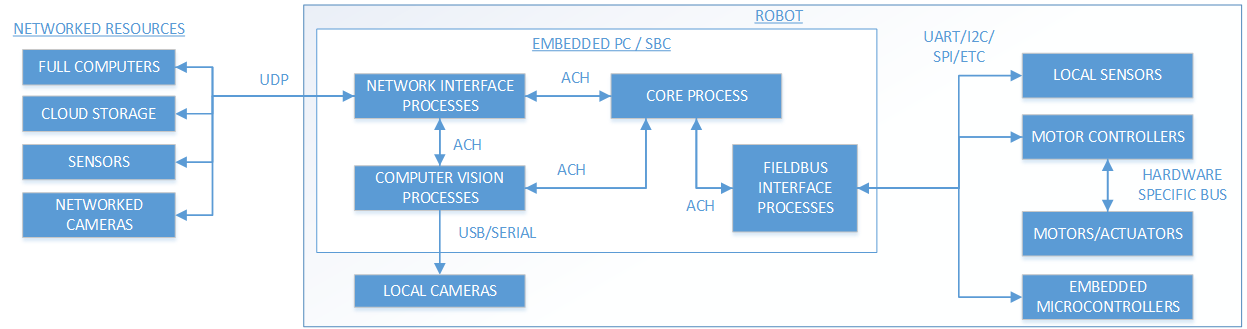
\includegraphics[width=2.0\columnwidth]{./images/idealsystem.png}
  \caption{Ideal System: Minimal Latency. This diagram shows how UDP and ACH IPC methods should be used for relevant system components.}
  \label{fig:idealsystem}
\end{figure*}

  Processing the large amount of messages into an ACH channel is critical to ensure usability of this method. This eliminates the issues of lost messages after the sockets buffer fills and prevents data obsolescence that would occur from a robot receiving data faster than it can process it. This method can be used with both UDP and TCP. The implementation of TCP is recommended with data integrity is of critical importance. For an ideal system that favors complete data transmission over increased latency then TCP should be utilized in conjunction with ACH. Figure \ref{fig:idealsystemtcp} details how an ideal system should be designed for data integrity.

\begin{figure*}[tbhp]
 \centering
 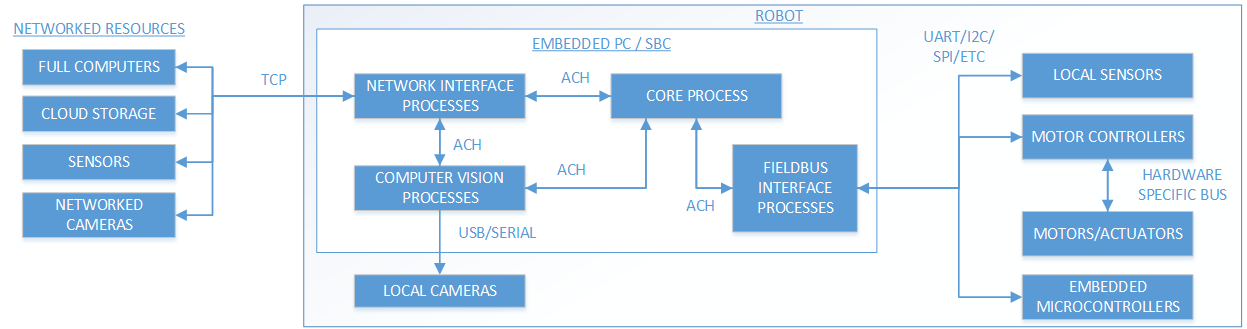
\includegraphics[width=2.0\columnwidth]{./images/idealsystem_integrity.png}
  \caption{Ideal System: Data Integrity. This diagram shows how TCP and ACH IPC methods should be used for relevant system components.}
  \label{fig:idealsystemtcp}
\end{figure*} 

The remaining IPC methods discussed in this paper should be used if a specific requirement dictates a specialized approach. The latency of a ZeroMQ message is detrimental to the real time operation of a robot. The only situation in which ZeroMQ should be implemented is when the system being designed requires a complex topology of processes that need to adhere to a publish/subscribe protocol. Robots are usually developed with a central command process that communicates with sub-processes, thus eliminating the advantages of ZeroMQ. 

ROS provides a vast library of modules to draw on for implementing hardware into the system. It is open source and supported on a wide variety of platforms. This reduces the amount of low level coding that needs to be written for each piece of hardware. This is advantageous for quickly building a system and reducing the amount of effort at the programming level. It fails to provide any real time support and the message latency and the head of line blocking nature of its TCP based messaging is problematic for high data transmission rates. ROS excels at building existing hardware and robotics into a viable system, but is not an ideal candidate for a custom built application.

While every robot is implemented differently, a combination of ACH channels and UDP/TCP sockets will be a viable application for the majority of systems. The flexibility and speed of the combined communication methods create a robust and modular link for real time robots to both internal and external components. 

\section{IMPLEMENTATION}

An example implementation of the information gathered is presented here. The objective of this design is to move blocks from an unknown starting location to a goal location. This is to be done remotely under user control with the only visual information coming from the robot. Visual information is collected via two webcams attached to a Raspberry Pi. The Raspberry Pi will receive commands from a remote terminal and control 4 servomotors by sending serial commands to the OpenCM motor controller. To achieve the required teleoperation, user input and both video feeds must be transmitted over a network.

The user will operate the robot with a joystick connected to a laptop. One process runs on the laptop to recieve information from the joystick and transmit to the robot over the network via UDP. UDP was selected for this communication link to ensure the fastest communication to the robot. Low latency was a priority as any lag in commands being received by the robot will proprogate to updating the video feedback and would make teleoperation difficult. Missed messages were of low concern as the frequency of message transmits would be replaced with new commands faster than the user can realize the delay. Command packets can be designed to be two bytes in size to minimize any risk of missed 

UDP was also selected for sending both video streams from the robot to be displayed on the user terminal. The video frame information required sending UDP messages at the maximum size limit for a single message. This did increase the probability of a message being missed, but the update rate of the video stream reduced on the impact of missed frames. As the video information is being interpreted by a human and not a computer, lower image resolution and frame rates were acceptable.

In order to have immediate response to user commands, the process collecting data from the joystick needed to operate at a high frequency. This will result in a large amount of messages being transmitted to the Raspberry Pi. Preliminary testing showed that while the user held the joystick down in a certain direction, a large quantites of the same command were stored in the robots UDP buffer. This would cause the robot to continue acting on outdated command information while it processed all received UDP commands. Increasing the update rate of the processes running on the PI to match incomming messages was not an acceptable solution as processing two USB video streams at higher rates was too taxing on the system. This led to errors and corruption of video information.

We needed to utilize the non head of line blocking aspect of the ACH IPC to access the most recent command message at a lower frequency. We incorporated an additional process that would receive UDP message and fill an ACH channel with data. This allowed the command process to update at a rate that matched the video information processed and sent back to the user without overloading the resouces of the Pi. Figure \ref{fig:cranebot block} shows a block diagram of the processes and communication methods for the robot.

\begin{figure}[thpb]
 \centering
 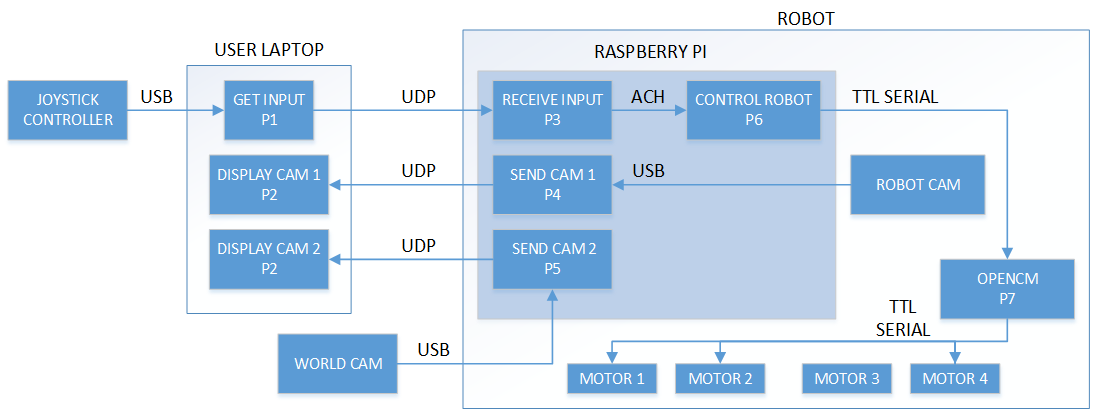
\includegraphics[width=1.0\columnwidth]{./images/cranebot2.png}
  \caption{Crane Robot Communication Diagram}
  \label{fig:cranebot block}
\end{figure} 

By evaluating the conceptual design and objective of this robot, we were able to narrow down the list of potential IPC methods to use. ZMQ would not be a viable candiate for use as the communication delay would be detrimental to the robots operation. There was no need for a complex communication topology as all of the process communication was between a single client/server pair. The Raspberry Pi and the OpenCM modules are single threaded processors and no additional synchronization features of ZMQ would be needed. ROS can be installed on the Pi and would have been possible candidate for use in this system except that the entire system would communicate with TCP at its core. The aforementioned head of line issue with command packets eliminates a sockets based approach for the entire system. Utilzing ACH and ACHD for network communications would allow us to achieve all of our design goals, but would require the user terminal to also have the ACH libraries to be installed. Utilizing sockets for the network communication was essential to build the most flexible system possible and allow for a modular input solution. This led to the combined solution of implemeneting both UDP and ACH for the robot. 

\section{CONCLUSIONS}

The selection of an IPC method for robotics must be done on a case by case basis by evaluating the design goals and intended implementation. Each of the IPCs discussed in this paper offer strenghts and weakenesses that the designer will need to accomodate. Code portability, data integrity, message latency, and system architecture all play an essential role in the selection process. While standarizing a communication protocol for the entire system may make implementation easier at the onset of a project, additional effort to optimize the system at a link by link level will vastly improve the operation of the robot. The results of the testing and research done in this paper conclude that combining different IPC methods within a robotic system allow for optimal message latency and flexibility of the system.

The ACH messaging system provides the ideal combination of speed and flexibility and should be utilized for internal messaging within a contiguous set of hardware. With the ability to configure an ACH channel as either blocking or non-blocking, the system can perform synchronously or asynchronously depending on the needs for the data. Additional configuration options allow the channel to be set as a FIFO or LIFO buffer without overwritting or losing any message data. The robot can access and react to the most recent sensor data while continuously logging the all data as it arrives. The sychronization provided internally by the data channels abstract the more complicted programming locks and allow for easitly implemented, thread safe operation on multicore robots. As multicore embedded SBCs become increasingly avaiable, ACH's synchronization allows for portability and upgradeablility between single and multicore systems.

The use of sockets, particularly UDP, is recommended for all network communication to and from the robot. Sockets is a standard POSIX library and its use allows for modular addition of sensors, controllers, and other networked systems. Robots often operate in a real time environment and message latency is of critical importance. This favors the use of UDP as a network IPC. UDP excels at fast one directional communication. Data packets can be designed to be small in size to reduce, if not eliminate, any issues of dropped messages. Additionally, the data rate can be increased to the point where any missed message are made irrelevant by new data before the robot would notice. Processing the large amount of messages into an ACH channel is critical to ensure usability of this method. This eliminates the issues of lost messages after the sockets buffer fills and prevents data obsolescence that would occur from a robot receiving data faster than it can process it.

The remaining IPC methods discussed in this paper should be used if a specific requirement dictates a specialized approach. The latency of a ZeroMQ message is detrimental to the real time operation of a robot. The only situation in which ZeroMQ should be implemented is when the system being designed requires a complex topology of processes that need to adhere to a publish/subscribe protocol. ZMQ would provide a simplified approach to transmitting a message to all desired recipients and the increased single transmit latency may be a superior option to manually chaining together ACH channel or Sockets client/servers. TCP does have the advantage of identifiying if messages are missed, but outside of a few datasets (data logging, position waypoints) high transmission rates superseed the need for 100"\%" data transmission. ROS provides a vast libary of modules to draw on for implementing hardware into the system. It is open source and supported on a wide variety of platforms. This reduces the amount of low level coding that needs to be written for each piece of hardware. This is advantageous for quickly building a system and reducing the amount of effort at the programming level. It fails to provide any real time support and the message latency and the head of line blocking nature of its TCP based messaging is problematic for high data transmission rates. ROS excels at building existing hardware and robotics into a viable system, but is not an ideal candidate for a custom built application.

While every robot is implemented differently, a combination of ACH channels and UDP sockets will be a viable application for the majority of systems. The flexibility and speed of the combined communcation methods create a robust and modular link for real time robots to both internal and external components. 


\addtolength{\textheight}{-12cm}   % This command serves to balance the column lengths
                                  % on the last page of the document manually. It shortens
                                  % the textheight of the last page by a suitable amount.
                                  % This command does not take effect until the next page
                                  % so it should come on the page before the last. Make
                                  % sure that you do not shorten the textheight too much.


%%%%%%%%%%%%%%%%%%%%%%%%%%%%%%%%%%%%%%%%%%%%%%%%%%%%%%%%%%%%%%%%%%%%%%%%%%%%%%%%
\section*{ACKNOWLEDGMENT}

placeholder for acknowledgements


%%%%%%%%%%%%%%%%%%%%%%%%%%%%%%%%%%%%%%%%%%%%%%%%%%%%%%%%%%%%%%%%%%%%%%%%%%%%%%%%
\nocite{*}
\bibliographystyle{IEEEtran}

\bibliography{IPC}

\end{document}
